\section{Auswertung}
\label{sec:Auswertung}

\subsection{Fehlerrechung}
\label{sec:Fehlerrechnung}

Alle Mittelwerte werden mit folgender Formel berechnet:

\begin{equation}
  \label{eqn:15}
  \overline{x} = \frac{1}{N} \sum_{i=1}^N x_i
\end{equation}

Der zugehörige Fehler des Mittelwertes berechnet sich mit:

\begin{equation}
  \label{eqn:16}
  \Delta \overline{x} = \frac{1}{\sqrt{N}} \sqrt{\frac{1}{N-1} \sum_{i=1}^N (x_i - \overline{x})^2}
\end{equation}

Im Folgenden wird die Gauß'sche Fehlerfortpflanzung für den neuen Fehler bei Nutzung fehlerbehaftete Größen in späteren Formeln genutzt:

\begin{equation}
  \label{eqn:17}
  \Delta f = \sqrt{ \sum_{i=1}^N (\frac{\partial}{\partial x_i})^2 \cdot (\Delta x_i)^2}
\end{equation}

Ausgleichsgeraden werden mit

\begin{align}
  y &= a \cdot x + b \\
  a &= \frac{\overline{xy}-\overline{x} \, \overline{y}}{\overline{x^2}-\overline{x}^2} \\
  b &= \frac{\overline{x^2}\overline{y}-\overline{x} \, \overline{xy}}{\overline{x^2}-\overline{x}^2}
\end{align}

berechnet. Die Regressionen, Ausgleichsgeraden und Fehler-Berechnungen werden mithilfe von Numpy, matplotlib und scipy durchgeführt.

\subsection{Bestimmung der Zeitkonstante}
\label{Zeitkonstante}

Aus den Daten aus Tabelle \ref{tab:zeitkonstante} soll nun die Zeitkonstante $\tau$ bestimmt werden.
Dafür wird aufgrund von

\begin{equation}
  ln\left(\frac{U_c}{U_0}\right) = -\frac{1}{RC}\,t
\end{equation}

eine lineare Regression zur Bestimmung der Zeitkonstante durchgeführt.
Die Messwerte, sowie die lineare Regression, wurden in Abbildung \ref{fig:zeitkonstante} aufgetragen.
Dafür wird folgende Formel genutzt:

\begin{align*}
  ln\left(\frac{U_c}{U_0}\right) &= -\frac{1}{a} t + b \\
  \text{mit } a &= \SI{0.2266707 \pm 0.009118}{ms}\\
  \text{und } b &= \SI{2.03602799 \pm 0.0427388}{V}
\end{align*}

Für die Zeitkonstante $\tau$ ergibt sich dann entsprechend der Steigung:
\begin{equation}
  \tau = RC = a = \SI{0.2266707 \pm 0.009118}{ms}
\end{equation}

\begin{table}
\centering
\caption{Messwerte zur Bestimmung der Zeitkonstante $\tau$ mit $U_0 = 1 = \text{const}$}
\label{tab:zeitkonstante}
\sisetup
{table-format=1.2}
\begin
{tabular}{S[table-format=3.0] S S[table-format=3.2]}
\toprule
{$t/10^{-4}\, \mathrm{s}$} &{$U_c/\,\mathrm{V}$} &{$ln\left(\frac{U_c}{U_0}\right)$} \\
\midrule
0.80 & 5.12 & 1.63\\
1.00 & 4.72 & 1.55\\
1.20 & 4.40 & 1.48\\
1.40 & 4.16 & 1.43\\
1.60 & 3.92 & 1.37\\
1.80 & 3.60 & 1.28\\
2.00 & 3.32 & 1.20\\
2.20 & 3.08 & 1.12\\
2.40 & 2.84 & 1.04\\
2.60 & 2.64 & 0.97\\
2.80 & 2.32 & 0.84\\
3.00 & 2.12 & 0.75\\
3.20 & 1.96 & 0.67\\
3.40 & 1.72 & 0.54\\
3.60 & 1.44 & 0.36\\
3.80 & 1.20 & 0.18\\
4.00 & 1.00 & 0.00\\
4.20 & 0.84 & -0.17\\
4.40 & 0.72 & -0.33\\
4.60 & 0.52 & -0.65\\
4.80 & 0.24 & -1.43\\
5.00 & 0.04 & -3.22\\
\bottomrule
\end{tabular}
\end{table}

\newpage

\begin{figure}[h]
  \centering
  \includegraphics{plot.pdf}
  \caption{Messwerte aus Tabelle \ref{tab:zeitkonstante} mit linearer Regression}
  \label{fig:zeitkonstante}
\end{figure}

Nun soll die Zeitkonstante ein zweites mal berechnet werden.
Zugrunde liegt hierbei die Spannungsamplitude A des Kondensators in Abhängigkeit zur Frequenz.
Dafür wird die Amplitude durch die Spannung $U_0$ geteilt und halblogarithmisch gegen die Frequenz in Abbildung \ref{fig:amplitude} aufgetragen.
Die zugrundeliegenden Messwerte sind aus Tabelle \ref{tab:amplitude} zu entnehmen.
Die nichtlineare Ausgleichsrechnung wir gemäß \eqref{eqn:13} durchgeführt und kann ebenfalls der Abbildung \ref{fig:amplitude} entnommen werden.
Die Zeitkonstante ergibt sich dann zu:
\begin{equation*}
  RC = \SI{-0.826 \pm 0.0071834}{ms}
\end{equation*}

\begin{table}
\centering
\caption{Amplitude der Kondensatorspannung mit Frequenz $\nu$}
\label{tab:amplitude}
\sisetup
{table-format=1.2}
\begin
{tabular}{S[table-format=3.5] S[table-format=3.5
]}
\toprule
{$\nu/\, \mathrm{Hz}$} &{$U_c/\,\mathrm{mV}$} \\
\midrule
10.00 &968\\
15.00 &975\\
30.00 &977\\
50.00 &954\\
80.00 &912\\
100.0 &878\\
140.0 &804\\
180.0 &729\\
210.0 &675\\
270.0 &583\\
300.0 &543\\
400.0 &438\\
500.0 &364\\
600.0 &309\\
700.0 &268\\
800.0 &237\\
900.0 &211\\
1000 &190\\
1500 &127\\
2000 &95\\
3000 &62\\
5000 &39.53\\
10000 &19.81\\
20000 &9.90\\
\bottomrule
\end{tabular}
\end{table}

\newpage

\begin{figure}[h]
  \centering
  \includegraphics{plot2.pdf}
  \caption{Messwerte aus Tabelle \ref{tab:amplitude} mit Ausgleichsrechnung zur Bestimmung der Zeitkonstanten}
  \label{fig:amplitude}
\end{figure}

Nun soll die Zeitkonstante ein drittes Mal mithilfe der Phasenverschiebung zwischen Generator- und Kondensatorspannung bestimmt werden.
Sie wird wie folgt berechnet:

\begin{equation}
  \phi = \frac{a}{b} \cdot 2\pi
\end{equation}

\begin{table}
\centering
\caption{Phasenverschiebung zwischen Eingangs- und Kondensatorspannung $\tau$}
\label{tab:phasenverschiebung}
\sisetup
{table-format=1.2}
\begin
{tabular}{S[table-format=3.5] S[table-format=3.5
]}
\toprule
{$\nu/\, \mathrm{Hz}$} &{$\phi/\,\mathrm{rad}$} \\
\midrule
10.00 &0\\
15.00 &0\\
20.00 &0.10\\
25.00 &0.13\\
30.00 &0.15\\
50.00 &0.25\\
100.0 &0.44\\
250.0 &0.85\\
500.0 &1.23\\
1000.0 &1.26\\
5000.0 &1.64\\
\bottomrule
\end{tabular}
\end{table}

\newpage

\begin{figure}[h]
  \centering
  \includegraphics{plot3.pdf}
  \caption{Messwerte aus Tabelle \ref{tab:phasenverschiebung} mit Ausgleichsrechnung zur Bestimmung der Zeitkonstanten}
  \label{fig:phase}
\end{figure}

\newpage

In Tabelle \ref{tab:phasenverschiebung} sind alle gemessenen Werte zu finden.
Diese Werte werden in Abbildung \ref{fig:phase} wieder mit einer Ausgleichsgeraden aufgetragen.
Die Ausgleichsgerade wird mithilfe der Gleichung \eqref{eqn:11} berechnet.

\begin{equation}
  RC = -0.0007474 \pm 5.3988 * \,10^{-5} \text{s}
\end{equation}

Nun soll die Beziehung der Relativamplitude $\frac{A(\omega)}{U_0}$ zu der Phase $\phi$ in einem Polarplot eingezeichnet werden.
Für die Theoriekurve wird die Formel:
\begin{align}
    \frac{A(\omega)}{U_0} &= -\frac{sin(\phi)}{\omega RC}
    \shortintertext{, sowie}
    sin(\phi) &= \frac{\omega RC}{\sqrt(1+\omega^2 R^2 C^2)}
\end{align}
verwendet.
Die restlichen Werte der Messpunkte können Tabelle \ref{tab:polar} entnommen werden.

\clearpage

\begin{table}
\centering
\caption{Phasenverschiebung zwischen Eingangs- und Kondensatorspannung $\tau$}
\label{tab:polar}
\sisetup
{table-format=1.2}
\begin
{tabular}{S[table-format=1.2] S[table-format=1.4]}
\toprule
{$\phi/\,\mathrm{rad}$} & {$\frac{A(\omega)}{U_0} $}\\
\midrule
0     & 0.9988 \\
0     & 0.9975 \\
0.10  & 0.9956 \\
0.13  & 0.9931 \\
0.15  & 0.9902 \\
0.25  & 0.9735 \\
0.44  & 0.9051 \\
0.85  & 0.6484 \\
1.23  & 0.3918 \\
1.26  & 0.2082 \\
1.64  & 0.0425 \\
\bottomrule
\end{tabular}
\end{table}

\begin{figure}[h]
  \centering
  \includegraphics{plot4.pdf}
  \caption{Messwerte aus Tabelle \ref{tab:polar} mit Theoriekurve}
  \label{fig:polar}
\end{figure}

\clearpage

\subsection{Der RC- Kreis als Integrator}
\label{sec:Integrator}

Es soll nun nachgewiesen werden, dass ein RC- Kreis auch als Integrator fungieren kann.
Dafür werden die berechneten Spannungen mit den gemessenen verglichen.
Bei den gemessenen Funktionen handelt es sich um Bildschirmaufnahmen.

\begin{align*}
  \shortintertext{Integration der Sinusspannung:}
  f(x) &= k \cdot sin(x) & F(x) &= k \cdot cos(x) \\
  \shortintertext{Integration der Dreieckspannung:}
  f(x) &=
  \begin{cases}
    k \cdot x, & -a < x \leq a \\
    -k \cdot x, & a < x \leq 3a
  \end{cases}
  & F(x) &=
  \begin{cases}
    \frac{k}{2} \cdot x^2, & -a < x \leq a \\
    -\frac{k}{2} \cdot x^2, & a < x \leq 3a
  \end{cases} \\
  \shortintertext{Integration der Rechteckspannung:}
  f(x) &=
  \begin{cases}
    k, & 0 < x \leq a \\
    -k, & a < x \leq 2a
  \end{cases}
  & F(x) &=
  \begin{cases}
    k \cdot x, & 0 < x \leq a \\
    -k \cdot x, & a < x \leq 2a
  \end{cases}
\end{align*}

Anhand dieser Figuren kann somit nachgewiesen werden, dass ein RC- Kreis auch als Integrator einer gegebenen Spannung fungieren kann.

\begin{figure}
  \centering
  \begin{subfigure}{0.48\textwidth}
    \centering
    \includegraphics[width=\textwidth]{build/plot5.pdf}
    \label{fig:sinplt}
  \end{subfigure}
  \begin{subfigure}{0.48\textwidth}
    \centering
    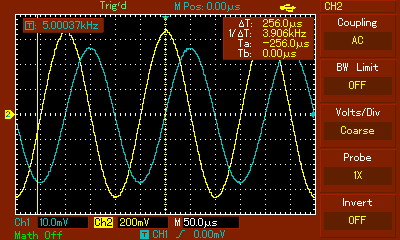
\includegraphics[width=\textwidth]{integration/MAP001.png}
    \label{fig:singms}
  \end{subfigure} \end{figure}

\begin{figure}
  \centering
    \begin{subfigure}{0.48\textwidth}
      \centering
      \includegraphics[width=\textwidth]{build/plot6.pdf}
      \label{fig:dreckplt}
    \end{subfigure}
    \begin{subfigure}{0.48\textwidth}
      \centering
      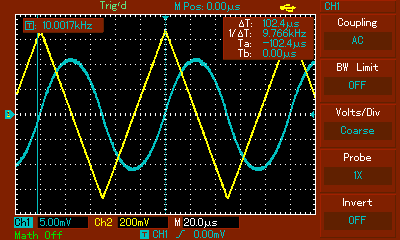
\includegraphics[width=\textwidth]{integration/MAP003.png}
      \label{fig:dreckgms}
  \end{subfigure} \end{figure}

  \begin{figure}
    \centering
    \begin{subfigure}{0.48\textwidth}
      \centering
      \includegraphics[width=\textwidth]{build/plot7.pdf}
      \label{fig:vierplt}
    \end{subfigure}
    \begin{subfigure}{0.48\textwidth}
      \centering
      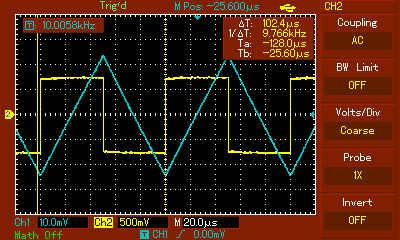
\includegraphics[width=\textwidth]{integration/MAP004.png}
      \label{fig:viergms}
    \end{subfigure} \end{figure}
